\documentclass[14pt]{extarticle}
% \documentclass[14pt]{article}

% \usepackage[style=authoryear,maxbibnames=9,maxcitenames=2,uniquelist=false,backend=biber,doi=false,url=false]{biblatex}
% \addbibresource{$BIB} % bibtex location
% \renewcommand*{\nameyeardelim}{\addcomma\space} % have comma in parencite
\usepackage{natbib}

\usepackage{xcolor}
\usepackage{amsmath}
\newcommand{\tuple}[1]{ \langle #1 \rangle }
%\usepackage{automata}
\usepackage{times}
\usepackage{ltablex}
\usepackage{tasks}

%%%%%% Template
\usepackage{hyperref}
\hypersetup{colorlinks=true,allcolors=blue}

\usepackage{vmargin}
\setpapersize{USletter}
\setmarginsrb{1.0in}{1.0in}{1.0in}{0.6in}{0pt}{0pt}{0pt}{0.4in}

% HOW TO USE THE ABOVE:
%\setmarginsrb{leftmargin}{topmargin}{rightmargin}{bottommargin}{headheight}{headsep}{footheight}{footskip}
%\raggedbottom
% paragraphs indent & skip:
\parindent  0.3cm
\parskip    -0.01cm

\usepackage{tikz}
\usetikzlibrary{backgrounds}

% hyphenation:
% \hyphenpenalty=10000 % no hyphen
% \exhyphenpenalty=10000 % no hyphen
\sloppy

% notes-style paragraph spacing and indentation:
\usepackage{parskip}
\setlength{\parindent}{0cm}

% let derivations break across pages
\allowdisplaybreaks

\newcommand{\orange}[1]{\textcolor{orange}{#1}}
\newcommand{\blue}[1]{\textcolor{blue}{#1}}
\newcommand{\red}[1]{\textcolor{red}{#1}}
\newcommand{\freq}[1]{{\bf \sf F}(#1)}
\newcommand{\datafreq}[2]{{{\bf \sf F}_{#1}(#2)}}

\def\qqquad{\quad\qquad}
\def\qqqquad{\qquad\qquad}

%%%%%%%%%%%%%%%%%%%%%%%%%%%%%%%%%%%%%%%%%%%%%%%%%%%%%%%%%%%%%%%%%%%%%%%%%%%%%%%%
%%%%%%%%%%%%%%%%%%%%%%%%%%%%%%%%%%%%%%%%%%%%%%%%%%%%%%%%%%%%%%%%%%%%%%%%%%%%%%%%

% fill-in-blank question style, found in https://tex.stackexchange.com/a/505089

\usepackage{ifthen}
\usepackage{tocloft}
\usepackage{exercise}
% \usepackage{xcolor}

% Set the Show Answers Boolean
\newboolean{showAns}
\setboolean{showAns}{false}
\newcommand{\showAns}{\setboolean{showAns}{true}}

% The length of the Answer line
\newlength{\answerlength}
\newcommand{\anslen}[1]{\settowidth{\answerlength}{#1}}

% ans command that indicates space for an answer or shows the answer in red
\newcommand{\ans}[1]{\settowidth{\answerlength}{\hspace{2ex}#1\hspace{2ex}}%
    \ifthenelse{\boolean{showAns}}%
        {\textcolor{red}{\underline{\hspace{2ex}#1\hspace{2ex}}}}%
        {\underline{\hspace{\answerlength}}}}%

\newcommand{\details}[1]{\settowidth{\answerlength}{#1}%
    \ifthenelse{\boolean{showAns}}%
        {\\ \textcolor{blue}{#1}}%
        {}}%

% Formatting how multiple choices Questions are formated.
\settasks{label=(\Alph*), label-width=30pt}


% Some commands for the Exercise Question package
\renewcommand{\QuestionNB}{\Large\protect\textcircled{\small\bfseries\arabic{Question}}\ }
\renewcommand{\ExerciseHeader}{} %no header
\renewcommand{\QuestionBefore}{3ex} %Space above each Q
\setlength{\QuestionIndent}{8pt} % Indent after Q number


% To create the list of answers with tocloft...
\newcommand{\listanswername}{Answers}
\newlistof[Question]{answer}{Answers}{\listanswername}

% Creates a TOC for Answers
\newcounter{prevQ}
\newcommand{\answer}[1]{\refstepcounter{answer}%
\ans{#1}%
\ifnum\theQuestion=\theprevQ%
        \addcontentsline{Answers}{answer}{\protect\numberline{}#1}% don't include the Q number
        \else%
        \addcontentsline{Answers}{answer}{\protect\numberline{\theQuestion}#1}%
        \setcounter{prevQ}{\value{Question}}%
        \fi%
        }%

% \hyphenpenalty=10000 % no hyphen
% \exhyphenpenalty=10000 % no hyphen
\sloppy              % hyphen

\newcommand{\HRule}{\rule{\linewidth}{0.5mm}}
\newcommand{\Hrule}{\rule{\linewidth}{0.3mm}}

%tocloft formatting listofanswers
\renewcommand{\cftAnswerstitlefont}{\bfseries\large}
\renewcommand{\cftanswerdotsep}{\cftnodots}
\cftpagenumbersoff{answer}
\addtolength{\cftanswernumwidth}{10pt}

\makeatletter% since there's an at-sign (@) in the command name
\renewcommand{\@maketitle}{%
  \parindent=0pt% don't indent paragraphs in the title block
  \centering
  {\Large \bfseries\textsc{\@title}} \\
  \vspace{5pt}
  {\large \textit{\@author}} \\
  \HRule \\
  \vspace{1em}
}
\makeatother% resets the meaning of the at-sign (@)


\title{ECON 2002.01 Final Exam}
\author{Hui-Jun Chen}


%%%%%%%%%%%%%%%%%%%%%%%%%%%%%%%%%%%%%%%%%%%%%%%%%%%%%%%%%%%%%%%%%%%%%%%%%%%%%%%%
%%%%%%%%%%%%%%%%%%%%%%%%%%%%%%%%%%%%%%%%%%%%%%%%%%%%%%%%%%%%%%%%%%%%%%%%%%%%%%%%
\begin{document}

\maketitle

\showAns
\listofanswer


% \includegraphics[width=\textwidth]{../QuestionBankImage/}

\begin{Exercise}

\Question (OUP-U13-Q16)
The figure shows that total investment spending can be volatile because the interaction of individual firms’ decisions can lead to vicious (low profit) or virtuous (high profit) circles. Which of the following might encourage all firms in the economy to behave in such a way that they all increase their investment spending together?
    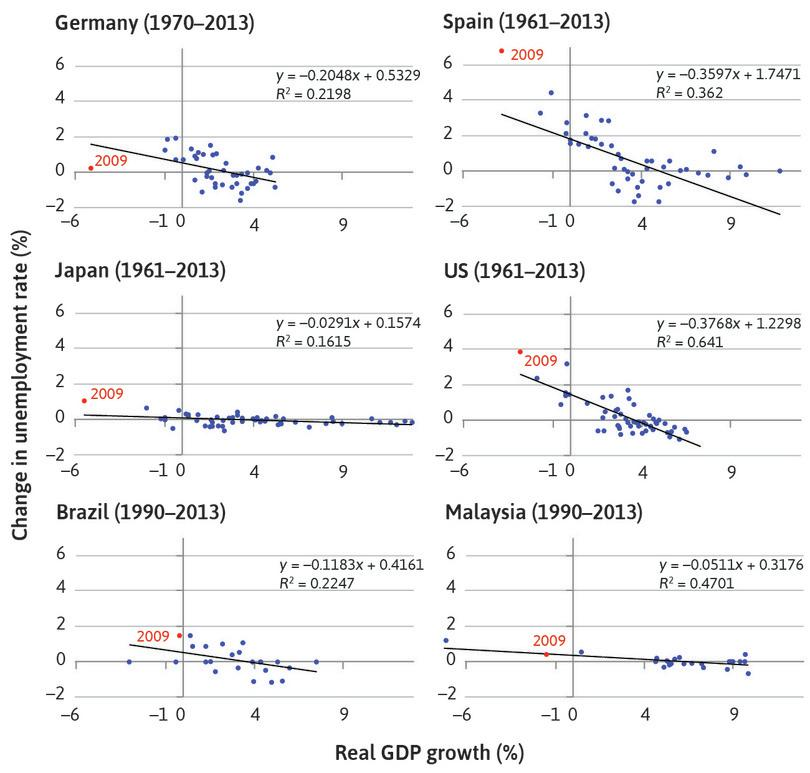
\includegraphics[width=\textwidth]{../QuestionBankImage/OUP-U13-Q7-01.jpg}
\answer{C}
\begin{tasks}(1)
    \task A fall in the exchange rate (the domestic currency becomes cheaper for foreign buyers).
        \details{This makes exports cheaper and imports dearer. Net exports are likely to increase and that will give boost to aggregate demand. But the positive effect will be limited to firms with significant exports and firms that have to buy materials from overseas will find their costs rising (and sales possibly falling).Also, fluctuations in exchange rates happen frequently. Any rise or fall is likely to be temporary. So a general boost to investment is unlikely.}
    \task A major technological breakthrough – say in batteries for electric cars.
        \details{Clearly, this is likely to encourage more investment in the automobile industry and in battery manufacture. Some firms may also recognise it as having implications for their industry even though they don’t make electric cars. But even with this ‘good news effect’ technological breakthroughs, however, general their application are unlikely to encourage all firms to expand investment simultaneously.}
    \task The use by government of fiscal policy to increase aggregate demand.
        \details{An increase in aggregate demand will encourage all firms to expect a higher demand for their products and this should have a beneficial effect on investment plans across the economy. This will be especially true if the policy is given lots of publicity and if the government’s promises are seen as credible.}
    \task Calls from government for firms to increase investment.
        \details{This is unlikely to have much effect. Firms undertake investment in order to remain competitive and/or to expand production. They do this because they see the possibility of profit and their shareholders will expect them to make the best decisions with respect to profit. Investments risky and firms are unlikely to undertake it just because governments ask them to do it. However, such encouragement might have some effect if combined with the publicity surrounding an expansionary fiscal policy.}
\end{tasks}
\newpage

\Question (OUP-U13-Q9)
The data for Spain suggests that Okun’s Law can be written as y = -0.3147x +1.2821, where y is the change in unemployment rate and x is the GDP growth rate. What is the predicted change in unemployment if GDP grows by 2 per cent?
\answer{C}
\begin{tasks}(1)
    \task Unemployment increases by 1.9115 percentage points.
        \details{1.9115 is the value we get if we ignore the negative sign on the coefficient. (1.2821 + 0.3147(2) = 1.9115).}
    \task Unemplyoment increases by 1.2758 percentage points.
        \details{1.2758 is the value we get if we enter 0.02 for 2 per cent, when the equation requires us to enter it as a whole number. (1.2821 – 0.3147(0.02) = 1.9115.}
    \task Unemployment increases by 0.6527 percentage points.
        \details{1.2821 -0.3147(2) = 0.6527}
    \task Unemployment increases by 1.2192 percentage points.
        \details{1.2192 is the value we get if we enter the growth rate as 0.2 instead of 2. 1.2821 - 0.3147(0.2) - 1.2192}
\end{tasks}
\newpage

\Question (OUP-U14-Q12)
In an economy where the MPC is 0.7, the proportional tax rate is 0.25 and the marginal propensity to import is 0.2, the multiplier will be:
\textit{Hint:} There's both MPC, proportional tax rate and MPI needs to be considered
\answer{C}
\begin{tasks}(1)
    \task 0.675
        \details{The value of the multiplier in this case is: 1/(1 - 0.7(0.75)) + 0.2 = 1/(1 - 0.525) + 0.2 = 1.48. 0.675 is the value of the multiplier if we omit the 1 in the numerator i.e. 0.475 + 0.2.}
    \task 2.1
        \details{The value of the multiplier in this case is: 1/(1 - 0.7(0.75)) + 0.2 = 1/(1 - 0.525) + 0.2 = 1.48. 2.1 is the value of the multiplier if we omit the marginal propensity to import.}
    \task 1.48
        \details{The value of the multiplier in this case is: 1/(1 - 0.7(0.75)) + 0.2 = 1/(1 - 0.525) + 0.2 = 1.48.}
    \task 2.35
        \details{The value of the multiplier in this case is: 1/(1 - 0.7(0.75)) + 0.2 = 1/(1 - 0.525) + 0.2 = 1.48. 2.35 is the value of the multiplier if we do the calculations in the wrong order, i.e. (1 - 0.7)0.75 + 0.2.}
\end{tasks}
\newpage

\Question (OUP-U14-Q10)
In the figure shown, a fall in output is caused by a reduction in investment. Which of the following would help restore output to its original level?
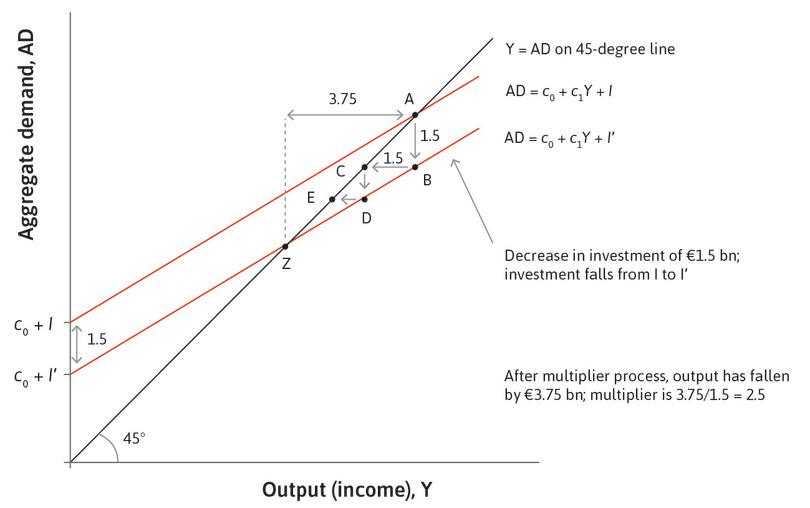
\includegraphics[width=\textwidth]{../QuestionBankImage/OUP-U14-Q10-01.jpg}
\answer{C}
\begin{tasks}(1)
    \task A reduction in autonomous consumption.
        \details{What is required is some compensating increase in aggregate demand. A reduction in autonomous consumption (the vertical axis intercept) will further reduce aggregate demand.}
    \task An increase in target wealth.
        \details{An increase in target wealth is likely to encourage households to save more, thus reducing aggregate demand.}
    \task An increase in actual wealth.
        \details{However, an increase in actual wealth may persuade them that there is less need to save. If so, consumption will increase and may compensate for the fall in investment.}
    \task A tightening of credit conditions.
        \details{A tightening of credit conditions will make borrowing more difficult, which will discourage consumption and may also encourage saving (which will also reduce consumption).}
\end{tasks}
\newpage

\Question (OUP-U15-Q22)
Assume that the central bank has an inflation target of 2\% per year but inflation is currently running at 4\%. The nominal policy (interest) rate is currently 5\%. The central bank needs to create a negative bargaining gap and estimates that the real policy rate required to achieve this is 3\%. Consequently it needs to set the nominal policy rate at:
\answer{B}
\begin{tasks}(1)
    \task 6\%.
        \details{No. If inflation is running at 4\% and the real rate needs to be 3\%, then according to the Fisher equation, the nominal rate needs to be 4\% + 3\% = 7\%.}
    \task 7\%.
        \details{According to the Fisher equation, 7\% is the required nominal rate.}
    \task 8\%.
        \details{No. If inflation is running at 4\% and the real rate needs to be 3\%, then according to the Fisher equation, the nominal rate needs to be 4\% + 3\% = 7\%.}
    \task 4\%.
        \details{No. The required rate is 4 + 3 = 7\%.}
\end{tasks}
\newpage

\Question (OUP-U15-Q20)
Assume that a bargaining gap remains constant at 1 per cent. The rate of inflation in future years will:
\answer{C}
\begin{tasks}(1)
    \task Remain constant at 1 per cent per year.
        \details{No. If there is a positive bargaining gap, there will be upward pressure on prices. This will be added to any existing rate of inflation, so the rate of inflation must accelerate.}
    \task Remain unchanged.
        \details{No. For the same reason, inflation must be accelerating.}
    \task Accelerate by 1 per cent per year.
        \details{Correct. If the bargaining gap is constant at 1 per cent, this will be added to the rate of inflation each year and so inflation will increase (accelerate) by 1 per cent per year.}
    \task Settle at 1 per cent.
        \details{No. So long as there is a bargaining gap, inflation cannot settle at any level. It must be accelerating or decelerating.}
\end{tasks}
\newpage

\Question (OUP-U16-Q6)
Last year, an economy had 1m registered unemployed and a labour force of 20m. Official statistics forecast a level of unemployment of 0.8m by the year’s end while the size of the labour force remains unchanged. If this happens then the unemployment rate will have:
\answer{B}
\begin{tasks}(1)
    \task Risen by 0.2m.
        \details{Incorrect. The level of unemployment has fallen by 0.2m. If the labour force is constant, then the rate of unemployment must also have fallen.}
    \task Fallen from 5 per cent to 4 per cent.
        \details{Correct. The unemployment rate has fallen from 1/20 (= 5\%) to 0.8/20 (= 4\%).}
    \task Fallen by 0.2m.
        \details{Incorrect. The level of unemployment has fallen by 0.2m, but the question asks about the rate.}
    \task Fallen by 0.2 per cent.
        \details{Incorrect. The level of unemployment has fallen by 0.2m but 0.2m is 1 per cent of 2m.}
\end{tasks}
\newpage

\Question (OUP-U16-Q20)
The figure shows long-run unemployment and real wage growth across the OECD. The rays drawn from the origin are described as ‘indifference curves’. This is because:
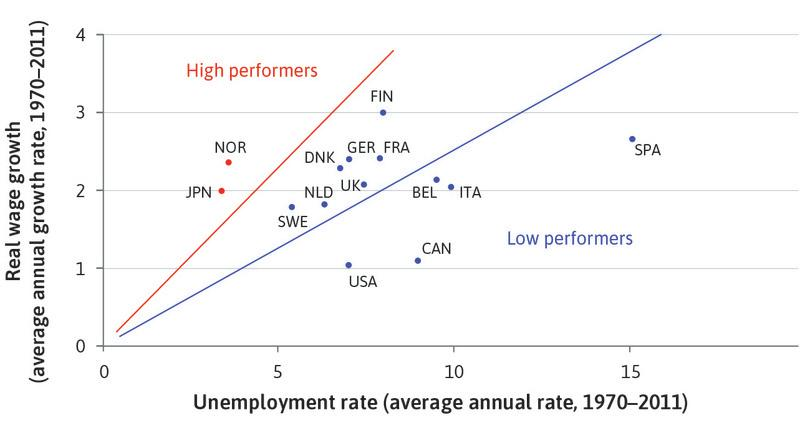
\includegraphics[width=\textwidth]{../QuestionBankImage/OUP-U16-Q20-01.jpg}
\answer{D}
\begin{tasks}(1)
    \task They show that people are indifferent to levels of unemployment.
        \details{Incorrect. ‘Indifferent to levels of unemployment’ would mean that they did not care about the level of unemployment. But an upward-sloping indifference curve means that people are prepared to accept higher unemployment only if real wages grow more rapidly.}
    \task They show a trade-off between unemployment and real wage growth.
        \details{Incorrect. A ‘trade-off’ means that more of something requires less of something else. But here, people are indifferent between combinations of high unemployment and high real wage growth, and low unemployment/low real wage growth. Therefore there is no trade-off involved.}
    \task They show that real wage growth and low unemployment go together.
        \details{`Incorrect. They show that real wage growth and high unemployment go together.}
    \task Each ray shows the combinations of unemployment and real wage growth that correspond to the same 'utility'.
        \details{An indifference curve shows combinations of two variables that give equal satisfaction. In the figure we can see that people can be equally happy with high or low unemployment, provided that higher unemployment is accompanied by higher real wage growth.}
\end{tasks}
\newpage

\Question (OUP-U17-Q11)
You are given the following information about the short-term nominal interest rate and the rate of inflation over a period of 8 years. In which year was the real rate of interest at its maximum and in which years might we regard monetary policy as having been expansionary?
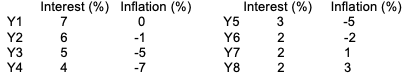
\includegraphics[width=\textwidth]{../QuestionBankImage/OUP-U17-Q11-01.png}
\answer{B}
\begin{tasks}(1)
    \task The real rate is at its maximum in Y4, but monetary policy is expansionary in all years since the rate of interest is falling.
        \details{The first part is correct. The real rate in Y4 is 11\% (= 4 - -7). However, the real rate has been rising since Y1 (7\%, 7\%, 10\%, 11\%) in spite of reductions in the nominal rate.	The real rate is at its maximum in Y4. It starts to fall in Y5 and falls below the Y1 rate in Y6.}
    \task Y6 is the earliest point at which we can describe monetary policy as expansionary.
        \details{The real rate is at its maximum in Y4. In spite of cuts to the nominal rate from Y1, the real rate does not fall below the rate in Y1 until we get to Y6 (= 4\%). The real rate does not turn negative until Y8.	The real rate is at its maximum in Y1 (= 7\%).}
    \task It only becomes negative in Y8, which is the earliest that we can describe policy as expansionary.
        \details{The real rate is higher in Y4 at 11\% (= 4 - -7). It is true that the real rate only becomes negative in Y8, but it falls below its initial (Y1) rate in Y6. We could argue that this reduction below the starting rate is where the expansionary policy starts.}
    \task The real rate is at its maximum in Y1 (=7\%) and monetary policy becomes expansionary in Y3 when the real rate falls to zero (= 5 - 5).
        \details{The real rate is at its maximum in Y4 at 11\% (= 4 - -7). In Y3, the real rate is actually 10\% (= 5 - -5). Note: we need to subtract a negative inflation rate.}
\end{tasks}
\newpage

\Question (OUP-U17-Q22)
The leverage ratio is defined as total assets/equity. Assume that a household’s sole asset is a house worth \$190,000, which it has bought with a mortgage loan of \$180,000. What is the value of the leverage ratio, and what happens to the ratio if the house value falls to \$185,000?
\answer{A}
\begin{tasks}(1)
    \task 19; 37.
        \details{The ratio begins at 19 (= 190/10) and rises to 37 (185/5) as the value falls. Notice how the small change in the value dramatically changes the ratio.}
    \task 19; 18.5.
        \details{The ratio begins at 19 (= 190/10) and rises to 37 (185/5) as the value falls. Remember, the ratio divides the value of the asset by the value of equity. As the value falls, both the value and the equity fall.}
    \task 0.053; 0.027.
        \details{These are the inverse of the correct values. Remember, the leverage ratio divides the asset value by the equity value, not the other way round.}
    \task 19; 13.
        \details{19 is correct for the initial value but 13 is the value of the ratio if the price increases by \$5,000 (to \$195,000) instead of falling to \$185,000. Note again though how the small change in value has a large effect on the ratio.}
\end{tasks}
\newpage



\Question (OUP-U13-Q21)
The Consumer Price Index (CPI):
\answer{C}
\begin{tasks}(1)
    \task Records the price of all goods and services in the economy.
        \details{Not all goods and services. It records the prices of what consumers actually buy and reflects the importance (or ‘weight’) of those items in the overall household budget.}
    \task Records the price of all goods produced in the domestic economy, including exports.
        \details{It records the prices of services as well. It also excludes the prices of exports (bought by overseas consumers) but does include the prices of imports.}
    \task Measures the general level of prices that consumers pay for goods and services.
        \details{It records the prices of goods and services in a typical ‘shopping basket’. The items and their weights are based upon a continuous sampling of consumer spending habits.}
    \task Measures the rate of inflation.
        \details{No. The CPI records the general level of prices. Inflation is the rate of change of prices.}
\end{tasks}
\newpage



\Question (OUP-U13-Q22)
The GDP deflator differs from the CPI in the following way:
\answer{C}
\begin{tasks}(1)
    \task It includes the price of exports.
        \details{The GDP deflator does records the prices of exports which are excluded from the CPI, but that is not the whole story.}
    \task It only records the prices of goods while CPI includes the price of services.
        \details{Both indicators include the prices of goods and services.}
    \task It includes the prices of exports but excludes the prices of imports.
        \details{The GDP deflator includes the price of exports but excludes the price of imports. This is the opposite of the CPI. Remember the GDP deflator is measuring the price of components of GDP, hence C + I + G  + X - M. By contrast, the CPI is measuring the prices of goods and services consumed by domestic residents.}
    \task The GDP deflator gives higher measures of inflation than the CPI.
        \details{There are various ways of measuring the price level and therefore the rate of inflation. The CPI and GDP deflator are just two (probably the most common). In some cases it is possible for an index to give biased (up or down) inflation rates compared with others. But that is not the case here. The CPI and GDP deflator will sometimes yield different results because they have slightly different components but there’s no reason to suppose that the differences show a bias in any one direction.}
\end{tasks}
\newpage



\Question (OUP-U13-Q24)
When a country’s GDP is being measured by the output method, the total figure comes to \$500bn. When measured by expenditure, we have the following components: Households’ spending on consumption = \$300bn, Firms’ spending on capital goods = \$50bn, Government spending on services = \$80bn, Government spending on capital goods = \$50bn, Government transfers (social security etc) = \$10bn, Exports = \$10bn and Imports = \$20bn. In the circumstances, how can we say the output and expenditure methods of calculating GDP are equivalent?
\answer{C}
\begin{tasks}(1)
    \task There is no problem. The expenditures sum to \$500bn which matches the output measure.
        \details{There is a problem. The expenditures sum to only \$490bn. (Remember, government transfers are not counted in the expenditure method since their spending will already be included in household consumption).}
    \task Both of these methods should give the same answer when calculated using real-world data.
        \details{In practice, it’s always likely that the three methods of calculating GDP will give slightly different answers because collecting the data is a massive task and firms do not keep records for the sole purpose of helping national income accountants. But in principle the answers should be the same. There appears to be \$10bn of expenditure which has not been recorded.}
    \task Adding to stocks of unsold goods is treated as a form of investment.
        \details{According to our figures, the economy produces \$500bn, but we can only trace \$490 of valid expenditure. This means that firms will be left with \$10bn of unsold goods and services. These will be recorded as ‘additions to stocks of unsold goods and raw materials’ as a sub-heading of investment.}
    \task Both methods of calculating GDP should always give the same answer in any circumstances.
        \details{In practice, it’s always likely that the expenditure and output method of calculating GDP will give slightly different answers because collecting the data is a massive task and firms do not keep records for the sole purpose of helping national income accountants. But in principle the answers should be the same. There appears to be \$10bn of expenditure which has not been recorded.}
\end{tasks}
\newpage


\Question (ECO-U13-Q1)
The following is the graph of the natural log of UK real GDP per capita between 1875 and 2014: Based on this information, which of the following statements is correct?
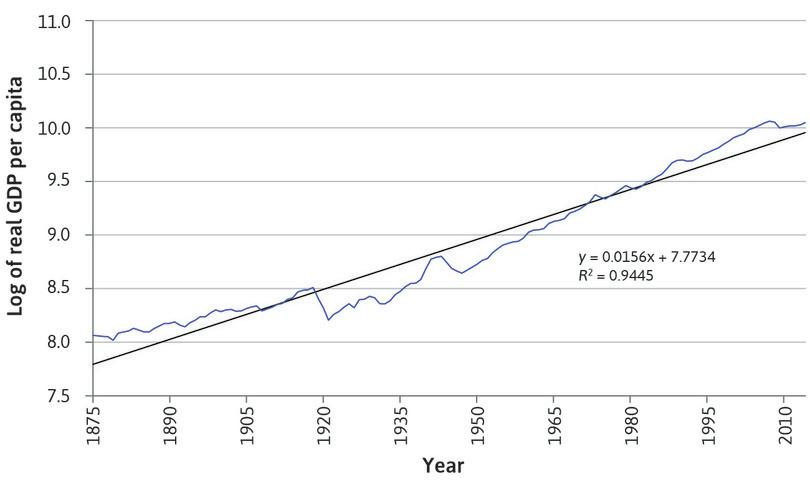
\includegraphics[width=\textwidth]{../QuestionBankImage/ECO-U13-Q1-01.jpg}
\answer{B}
\begin{tasks}(1)
    \task The graph shows that real GDP per capita in the UK in 1955 was about £8,000.
        \details{The graph shows that the natural log of GDP per capita in the UK in 1955 was about 8.9, that is, ln(GDP per capita) = 8.9. This means that GDP per capita = e8.9 = £7,332. (It was, in fact, e8.91 = £7,370.)}
    \task The slope of the best-fit straight line is the average annual growth rate.
        \details{This is stated in Figure 13.2, Section 13.1.}
    \task The graph shows that the average growth rate was lower in the decades after 1921 than in the decades before 1918.
        \details{While the log of real GDP per capita was lower immediately after 1921 than before 1918, the slope of the log graph is steeper. This means that the growth rate was higher after 1921 than before 1918.}
    \task The graph of real GDP per capita plotted using a ratio scale would look very different to the graph above.
        \details{The graph of real GDP per capita plotted using a ratio scale would look the same as the graph of the natural log of real GDP per capita plotted on a linear scale.}
\end{tasks}
\newpage



\Question (OUP-U14-Q4)
Assume that the level of consumption in an economy is given by the expression 1000 + 0.7Y, when Y = 50,000, consumption will be:
\answer{B}
\begin{tasks}(1)
    \task 35,000
        \details{If Y = 50,000, then 0.7Y = 35,000. But the consumption function requires us to include the additional 1,000.}
    \task 36,000
        \details{If Y = 50,000 then 1,000 + 0.7Y = 1,000 + 35,000 = 36,000.}
    \task 166,666
        \details{166,666 = 50,000/0.3, which is income divided by the marginal propensity to save.}
    \task 72,428
        \details{72,428 = 1,000 + (50,000/0.7). Consumption is calculated as 1,000 + (50,000 x 0.7).}
\end{tasks}
\newpage



\Question (OUP-U14-Q19)
The ‘paradox of thrift’ is an example of:
\answer{B}
\begin{tasks}(1)
    \task A contradiction in terms.
        \details{No contradiction is involved.}
    \task The fallacy of composition.
        \details{The paradox of thrift is an example of a ‘fallacy of composition’ because what is true in the individual case does not hold when applied at the population level (individual actions are ‘composed’ or put together). In this case an individual can save more but if everyone does it, income consumption and saving fall.}
    \task Positive feedback.
        \details{Positive feedback refers to a process whereby an initial disturbance creates a chain of events that eventually encourages a further disturbance of a similar kind. It is not relevant here.}
    \task Negative feedback.
        \details{Positive feedback refers to a process whereby an initial disturbance creates a chain of events that eventually encourages a further disturbance that cancels or offsets the initial disturbance. It is not relevant here.}
\end{tasks}
\newpage




\Question (TEA-U14-Q1)
The diagram depicts a consumption function of an economy, where $ C $ is the aggregate consumption spending, $ Y $ is the current income of the economy, and $ c_0 $ is the fixed (or autonomous) consumption such that $c_0 > 0$. Assume that households that are not credit-constrained would completely smooth their consumption. Which of the following statements is correct?
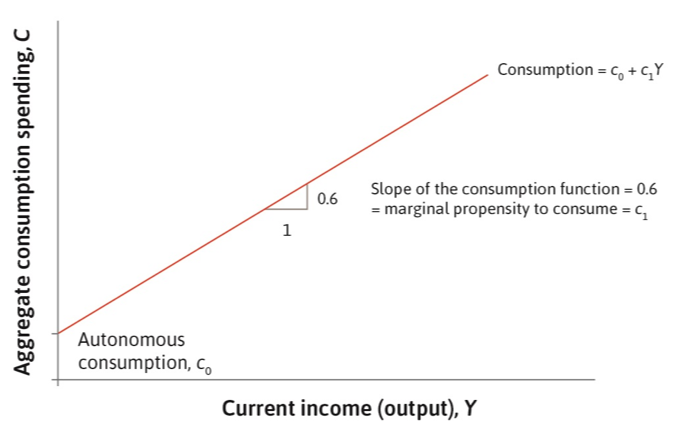
\includegraphics[width=\textwidth]{../QuestionBankImage/TEA-U14-Q1-01.png}
\answer{A}
\begin{tasks}(1)
    \task If all households were not credit-constrained, and all income changes were perceived to be temporary, then the aggregate consumption line would be horizontal.
        \details{In this case, all households can completely smooth consumption and would not react to temporary changes in income, so the aggregate consumption line would be horizontal.}
    \task During a credit crunch when the banks become less willing to lend, the aggregate consumption line would become flatter.
        \details{In a credit crunch, more households would become credit-constrained so their marginal propensity to consume would increase. Therefore the line would become steeper.}
    \task If a higher proportion of households have 'weakness of will', then the aggregate consumption line would be flatter.
        \details{Weakness of will' means that when there is an expected fall in income, the households are less likely to adjust their consumption ahead of the fall, in order to build up some savings so that they can smooth consumption. In this case their marginal propensity to consume would be higher, implying a steeper aggregate consumption line.}
    \task If the current income falls to zero, there will be zero consumption.
        \details{$c_0 > 0$ means that even if the current income is zero, the households will consume a strictly positive amount.}
\end{tasks}
\newpage



\Question (TEA-U14-Q2)
Assuming that there is no government spending or trade, an economy’s aggregate demand is given by its domestic consumption ($ C $) and investment ($ I $), $AD = C+  I= c_0+ c_{1}Y+ I$. In the economy’s goods market equilibrium this equals its output: $AD = Y$. Solving for $ Y $ this yields: $Y = [1/(1 - c_1)] (c_0 + I)$. Given this equation, which of the following statements is correct?
\answer{B}
\begin{tasks}(1)
    \task The multiplier is given by $1 – c_1$.
        \details{The multiplier is given by $1/(1 – c_1)$.}
    \task The boost in the economy’s output is the same, regardless of whether the aggregate demand shock comes from an increase in investment Ior in autonomous consumption $ c_0 $.
        \details{The same multiplier ($1/(1 – c_1)$) applies to both autonomous consumption and investment.}
    \task The larger the marginal propensity to consume ($ c_1 $), the smaller the multiplier.
        \details{A larger $ c_1 $ means a smaller $1 – c_1$, which in turn means a larger multiplier $1/(1 – c_1)$.}
    \task If $c_1= 1/3$, then a £1 million increase in investment would result in a £2 million increase in output, ceteris paribus.
        \details{When $c_1= 1/3$, then $1/(1 – c_1) = 1.5$, and therefore a £1 million increase in I would result in a £1.5 million increase in Y.}
\end{tasks}
\newpage



\Question (OUP-U14-Q21)
Insert the correct combination of terms in the following sentence: ‘The budget deficit refers to…., while government debt refers to…..’
\answer{C}
\begin{tasks}(1)
    \task Households’ borrowing; government borrowing.
        \details{A ‘budget deficit’ could in principle describe any situation where expenditure exceeded revenue, including a household’s accounts, but in economic terms, ‘the budget deficit’ refers to the deficit in the government’s accounts.}
    \task Firms’ borrowing; government borrowing.
        \details{A ‘budget deficit’ could in principle describe any situation where expenditure exceeded revenue, including a household’s accounts, but in economic terms, ‘the budget deficit’ refers to the deficit in the government’s accounts.}
    \task The government’s current borrowing requirement; the accumulation of past government borrowing.
        \details{The ‘budget deficit’ refers to the borrowing (if any) that results from the government’s excess of expenditure over revenue in a particular year. It is a flow and needs to be measured over time. ‘Government debt’ refers to the accumulation of past deficits. In layman’s terms this is what most people refer to as the ‘national debt’. It is a stock and is measured at a point of time.}
    \task Consumer credit; the national debt.
        \details{‘Consumer credit’ is a vague term which could refer to the current borrowing by households (usually excluding mortgages) or to their total indebtedness accumulated over years. Either way, it is a reference to households, while the question is focused on government accounts.}
\end{tasks}
\newpage



\Question (OUP-U15-Q4)
At the end of 2015 the UK consumer price index was 258; at the end of 2016 it was 267. According to this information, the annual rate of inflation during 2016 was approximately:
\answer{A}
\begin{tasks}(1)
    \task 3.3 percent.
        \details{Correct. If the price index has risen from 258 to 267, it has risen by 9 points and 9/258 = 0.033 or 3.3 per cent.}
    \task 9 percent.
        \details{Although the index changed by 9 points, to calculate a percentage change we need to take account of the starting value.}
    \task 2.67 percent.
        \details{267 (but not 2.67) is the final level of the index, but it is the change that we are interested in.}
    \task 0.33 percent.
        \details{The decimal point is in the wrong place. The answer is 0.033 or 3.3 per cent.}
\end{tasks}
\newpage



\Question (OUP-U15-Q6)
An overseas bank announces that it is introducing a new type of savings account that pays a 3\% fixed rate of interest for deposits of a one year duration. This 3\% is:
\answer{C}
\begin{tasks}(1)
    \task A real rate of interest.
        \details{For this to be a real rate of interest we would need to know the rate of inflation since the real rate = nominal rate – inflation.}
    \task A post-tax rate of interest.
        \details{Tax is normally due on interest received (since it is a form of income). It could be the case that the bank pays tax on our behalf before giving us the interest, but that is unusual and there is no suggestion of it here, so we have to assume that this is a ‘gross’ rate of interest on which we shall have to pay tax later.}
    \task A nominal rate of interest.
        \details{It is the nominal rate of interest.}
    \task A long-term rate of interest.
        \details{Since the interest is paid for only one year, we can hardly call it a long-term rate of interest. ‘Long-term’ has no fixed definition, but in finance it would normally be taken to mean 10 years or more (definitely not one year).}
\end{tasks}
\newpage



\Question (OUP-U15-Q14)
Imagine that at the end of 2014 your monthly income in money terms was £2000 per month while the index of retail prices was 100. At the end of 2015, your monthly income was £2100 while the index of retail prices was 110. During 2015, your real income had:
\answer{D}
\begin{tasks}(1)
    \task Increased by £100.
        \details{No. It is your nominal income that has increased by £100.}
    \task Fallen by 10 percent.
        \details{It has fallen but by less than 10 per cent, since prices have risen by 10 per cent but you have received some increase in nominal income to offset this.}
    \task Increased by 5 percent.
        \details{No. It is your nominal income that has increased by 5 percent (100/2000).}
    \task Fallen by 5 percent.
        \details{Your real income has fallen by 5 per cent, since the price level has risen by 10 per cent but your money has increased by only 5 per cent.}
\end{tasks}
\newpage



\Question (OUP-U15-Q24)
In a severe recession, with falling prices, the economy may need a negative real interest rate in order to give sufficient stimulus to aggregate demand. What particular problem for conventional monetary policy do negative real interest rates pose?
\answer{D}
\begin{tasks}(1)
    \task A negative real rate of interest redistributes income from savers to borrowers.
        \details{It is true that a negative real rate redistributes income from lenders to borrowers, since lenders are effectively paying borrowers to borrow. This is a consequence but not the main practical problem for policymakers.}
    \task A negative real rate of interest may cause an asset price boom.
        \details{It is always possible that a low interest rate may cause an asset price boom. However, this problem is not specific to negative real rates, and if the economy is in a severe recession an asset price boom may be helpful if it encourages additional household spending. So this is not the main problem.}
    \task A negative real rate of interest may encourage reckless borrowing.
        \details{This is always a risk when interest rates are low (not necessarily negative). From the point of view of a recession, reckless borrowing may be helpful if it increases aggregate demand, though the effects for the borrowers may of course be regrettable.}
    \task The policy rate needs to be more negative than the rate of deflation but nominal rates cannot go below zero.
        \details{This is the real problem. If the rate of inflation falls to zero and the economy requires a stimulus, it may need a rate of interest below zero. But it is very difficult to see how a negative rate of interest could be imposed. The moment that assets begin to pay negative rates (meaning that their holders are paying borrowers), their holders will sell and hold notes and coins instead.}
\end{tasks}
\newpage



\Question (TEA-U15-Q2)
Consider a scenario where the Bank of England views the UK economy to be overheating and is attempting to slow the economy down using monetary policy. Which of the following statements regarding the effects of an interest rate rise is correct?
\answer{B}
\begin{tasks}(1)
    \task It leads to higher bond prices, which results in higher demand for UK bonds.
        \details{An interest rate rise does lead to higher demand for UK bonds, but due to their lower prices.}
    \task It leads to higher demand for GBP, which results in an appreciation of the GBP.
        \details{Higher interest rates attract international investors, which in turn raises demand for GBP.}
    \task It leads to the UK exports becoming cheaper and imports becoming more expensive.
        \details{Higher interest rates lead to lower bond prices, resulting in higher demand for UK bonds. This in turn leads to a GBP appreciation, making UK imports cheaper and exports more expensive, which depresses aggregate demand in the UK.}
    \task It has opposing effects on the UK’s aggregate demand (AD): it discourages investment, which lowers AD, but results in cheaper imports, which boosts AD.
        \details{Cheaper imports mean greater leakages from the domestic economy. This reduces aggregate demand.}
\end{tasks}
\newpage



\Question (OUP-U16-Q17)
We expect the diffusion of new technology to raise both the real wage and the level of employment. But this takes time, during which some people may lose out. These include:
\answer{A}
\begin{tasks}(1)
    \task Older, less-adaptable, workers.
        \details{Correct. The introduction of new technology may require workers with skills that are different from those previously required. If existing workers are to continue, some degree of retraining will be required and this involves costs, both to the firms and the workers. With older workers, there are fewer years with which to recover the costs of retraining through their higher output. This may discourage firms from undertaking the investment in retraining. These workers also may feel that they will not have long enough to earn the higher real wage to make the effort of retraining worthwhile.}
    \task Firms with far-sighted management.
        \details{Incorrect. Firms with far-sighted management (and their workers) will probably have been able to plan ahead. More highly-skilled workers may already have been recruited. The choice of retraining or early-retirement may already have been offered to older or less-skilled workers. For these firms, the introduction of new technology will be less disruptive.}
    \task Young, mobile, workers.
        \details{Incorrect. Young workers tend to be easier to retrain (having left full-time education more recently). They also have more years over which to earn the benefits of their new skills. If they decide against retraining but they are mobile, then they can move to other places in order to use their existing skills elsewhere.}
    \task Workers in essential services.
        \details{Incorrect. Workers in essential services are unlikely to lose out because their employers will be under great pressure to retain them. This means they will have to offer retraining facilities and future conditions of employment that provide a strong incentive for existing workers to stay and enjoy the benefits of the new technology.}
\end{tasks}
\newpage




\Question (OUP-U16-Q12)
Suppose that the productivity of labour ($\lambda$) is \$35,000 per year and the equilibrium mark up ($\mu$) is 0.25. The long-run price-setting curve will be at a real wage of:
\answer{B}
\begin{tasks}(1)
    \task \$8,750.00
        \details{Incorrect. The real wage will be $(1- \mu) \times $ productivity or $\lambda$; in this case $0.75 \times  \$35,000$. \$8,750 is 0.25 x \$35,000.}
    \task \$26,250.00
        \details{Correct. \$26,250 is $0.75 \times  \$35,000$.}
    \task \$46,666.00
        \details{Incorrect. \$46,666 is the result of increasing \$35,000 by 0.25. We need to take the equilibrium markup into account.}
    \task \$61,250.00
        \details{Incorrect. \$61,250 is the result of increasing \$35,000 by 0.75. We need to take the equilibrium markup into account.}
\end{tasks}
\newpage



\Question (OUP-U16-Q18)
Which of the following might help to minimise the costs of adapting to new technology?
\answer{B}
\begin{tasks}(1)
    \task Strict regulation of new start-ups.
        \details{Incorrect. Regulations that deter new firms from starting up do not lower the costs of adapting to new technology, but rather they discourage the new technology being introduced in the first place.}
    \task Government re-training schemes.
        \details{Government-funded schemes that help workers retrain in order to work with the new technology reduce the costs to workers who might otherwise be unemployed.}
    \task A poorly developed financial sector.
        \details{Incorrect. A poorly developed financial sector might it difficult for new firms to raise start-up capital and established firms to raise capital for replacement investment. Both of these serve to discourage the introduction of the new technology rather than the costs that flow from it.}
    \task A shortage of skilled labour.
        \details{Once again, a shortage of skilled labour may deter innovation. The shortage does nothing to lower the costs of technological change once it has occurred.}
\end{tasks}
\newpage



\Question (TEA-U17-Q3)
The diagram describes the general movements in employment, profits, and wages in the 1950s to 1970s, using the labour market model. In addition, note that the postwar accord collapsed in the US in the 1960s, while it survived in Sweden. Which of the following statements regarding this period is correct?

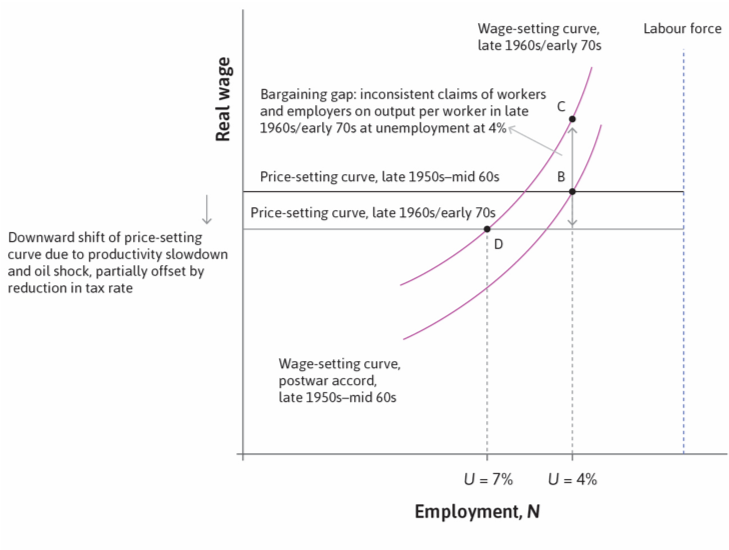
\includegraphics[width=\textwidth]{../QuestionBankImage/TEA-U17-Q3-01.png}
\answer{C}
\begin{tasks}(1)
    \task With less powerful trade unions, the wage-setting curve in the US rapidly fell back, leading to lower wages and higher unemployment.
        \details{Despite having less powerful trade unions, workers in the US nonetheless managed to defend their share of the pie, now shrunken by the oil price hike. This led to the wages remaining above the new lower price-setting curve, causing stagflation.}
    \task With a powerful centralised labour movement, the wage-setting curve was kept high in Sweden, causing high wage demand, low profits, and low unemployment.
        \details{As noted, the postwar accord survived in Sweden. This meant that wage claims were restrained to preserve profitability, investment, and high levels of employment.}
    \task Due to the strong bargaining position of workers, the oil shock primarily hit employers, redistributing income from profits to wages, causing an end to the fair-shares bargaining (the postwar accord) in the US.
        \details{Since workers defended their share of the pie, after the oil shocks, wages were above the price setting curve, which reduced profits, investment and productivity growth.}
    \task The golden age ended because of aggregate demand problems, caused by the oil shocks of the 1970s.
        \details{The Golden Age ended because of problems on the supply side of the economy, with lower investment and lower productivity growth.}
\end{tasks}
\newpage



\Question (OUP-U17-Q5)
Based on the information in Figures 17.2 and 17.3, which of the following statements about the rate of profit and net investment in the golden age (1948-73) and the great moderation (1979-2008) could be true?

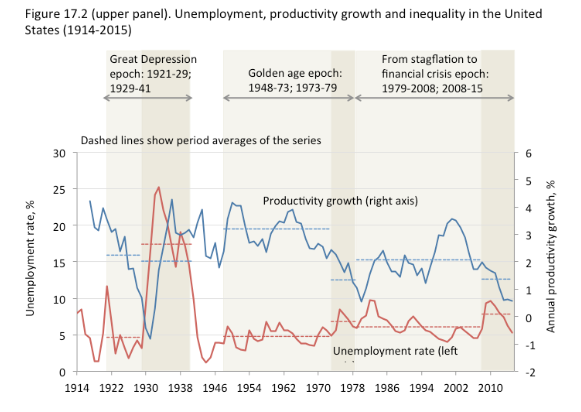
\includegraphics[width=\textwidth]{../QuestionBankImage/OUP-U17-Q5-01.png}
\answer{A}
\begin{tasks}(1)
    \task Productivity growth is more rapid in the golden age and so we would expect to see a higher level of net investment. Investment is likely to be encouraged by high profits.
        \details{Productivity growth comes from the implementation of new technology, which is embodied in new capital equipment. Figure 17.3 confirms that the growth in the capital stock (net investment) was also higher in the golden age, as was the post-tax profit rate.	Productivity growth is more rapid in the golden age, so we would expect to see a higher level of net investment.}
    \task This higher level of investment will leave smaller profits.
        \details{The first part of the answer is correct, but profit is calculated after the expenditure on new capital equipment. It is the fact that additional capital adds to profit that makes investment attractive.	Productivity growth appears to have been about 20\% per year in the golden age and 15\% per year during the later great moderation.}
    \task We would thus expect to see higher net investment in the golden age.
        \details{Firstly, the numbers are wrong. 20\% and 15\% refer to the unemployment rate (left hand scale), not productivity growth (right hand scale). The correct rates were about 3.2\% per year and 2\% per year. You would be correct in expecting higher net investment in the golden age, which is confirmed by Figure 17.3. But this statement says nothing about the rate of profit in either period.	If net investment were high, we would expect this to be a result of firms being unable to make a profit using the old equipment.}
    \task Profits would therefore be lower and net investment higher in the golden age compared to the great moderation.
        \details{The second part is correct – higher productivity growth goes with higher net investment. However, while individual firms may be compelled to improve their performance by introducing new technology, we would only expect a general (or aggregate) increase in capital spending if profits in general were high.}
\end{tasks}
\newpage



\Question (OUP-U17-Q23)
Following the collapse of Lehman Brothers in September 2008, some of its managers blamed the US government for putting pressure on banks to lend to subprime borrowers. What effect do you think this had on the household leverage ratios and on the financial risks faced by subprime borrowers?
\answer{B}
\begin{tasks}(1)
    \task Leverage ratios rose as banks accepted smaller deposits, but the risk of a fall/rise in house prices is unchanged.
        \details{The first part is correct. As banks sought out poorer and poorer customers, they had to accept smaller deposits/collateral and leverage ratios rose. This in itself has no effect on the probability of a change in housing prices, but for all subprime borrowers, the financial risk of falling into negative equity is greater with a high leverage ratio than a low one.	Banks felt obliged to accept lower levels of collateral, so households began with smaller housing equity and higher leverage ratios.}
    \task This made them more vulnerable to a fall in house prices.
        \details{Poorer households started with smaller equity and higher leverage ratios. This meant that a small price fall would push them into negative equity.}
    \task Leverage ratios fell and the risk to households increased.
        \details{Leverage ratios rose (remember the formula). Households consequently faced higher risk of negative equity from small price movements.}
    \task Leverage ratios rose but the effect on the risks faced by subprime borrowers is ambiguous (may increase or decrease depending on the household).
        \details{The first part is correct. It is also true that different households will have different attitudes to risk, different skills in managing it, and will put different priorities on their determination to cope with adverse shocks. However, for all subprime borrowers, the risk of falling into negative equity is greater with a high leverage ratio than a low one.}
\end{tasks}

\end{Exercise}

\end{document}
